\documentclass[a4paper]{article}
\usepackage{latexsym,amssymb,amsmath,amsbsy,amsopn,amstext,xcolor,multicol}
\usepackage{ctex,hyperref,graphicx,wrapfig,fancybox,listings}
\usepackage{pgf,pgfarrows,pgfnodes,pgfautomata,pgfheaps,pgfshade}
\usepackage[top=1in, bottom=1in, left=1.25in, right=1.25in]{geometry}
\graphicspath{{pic/}}
\title{\bf 网安实验-第一周}
\date{2017.10}
\author{计64~翁家翌~2016011446}
\begin{document}
\kaishu
\ttfamily
\maketitle
%\tableofcontents
%\newpage
\section{问题1}
一个局域网内部的两台计算机A、B的子网应该是192.168.26.0/24,网关192.168.26.2,其中B的子网掩码本应该是255.255.255.0,被不小心配成了了255.255.255.224。请问A和B之间能否通信?在A上ping B的地址,或者从B上ping A的地址,测试他们之间的连通性;同时,使用Wireshark或tcpdump捕获ICMP和ARP的流量,分析通或不通的原因。
\subsection{实验步骤}
将路由器TP-Link的网关设置成\uline{192.168.26.1},Mac地址为\uline{80:89:17:10:a4:68},并在路由器内配置两台机器的静态路由分别为\uline{192.168.26.3/27}(本机,Mac为\uline{18:5e:0f:18:0f:ec})和\uline{192.168.26.129/24}(对方,Mac为\uline{98:e0:d9:7b:50:4b})。

对方使用命令\uline{ping 192.168.26.3},显示无法ping通;本机使用命令\uline{ping 192.168.26.129},前两次收到了Redirect的消息,后面能够ping通,与此同时对方也能够正常ping通。

使用Wireshark抓包,数据如下:
\begin{figure}[htp]
\centering
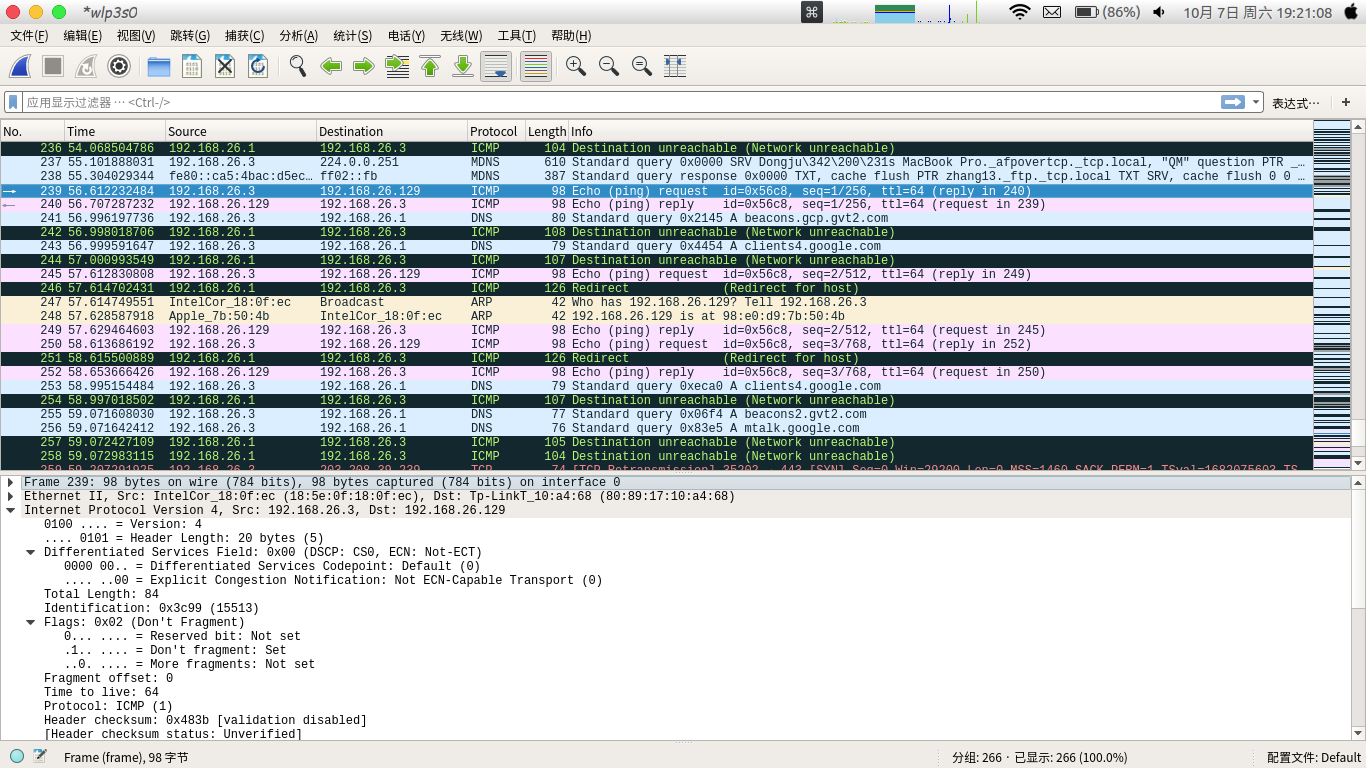
\includegraphics[width=1.0\linewidth]{tplink-mac.png}
\caption{ping seq=1/256}
\label{fig:1}
\end{figure}

\begin{figure}[htp]
\centering
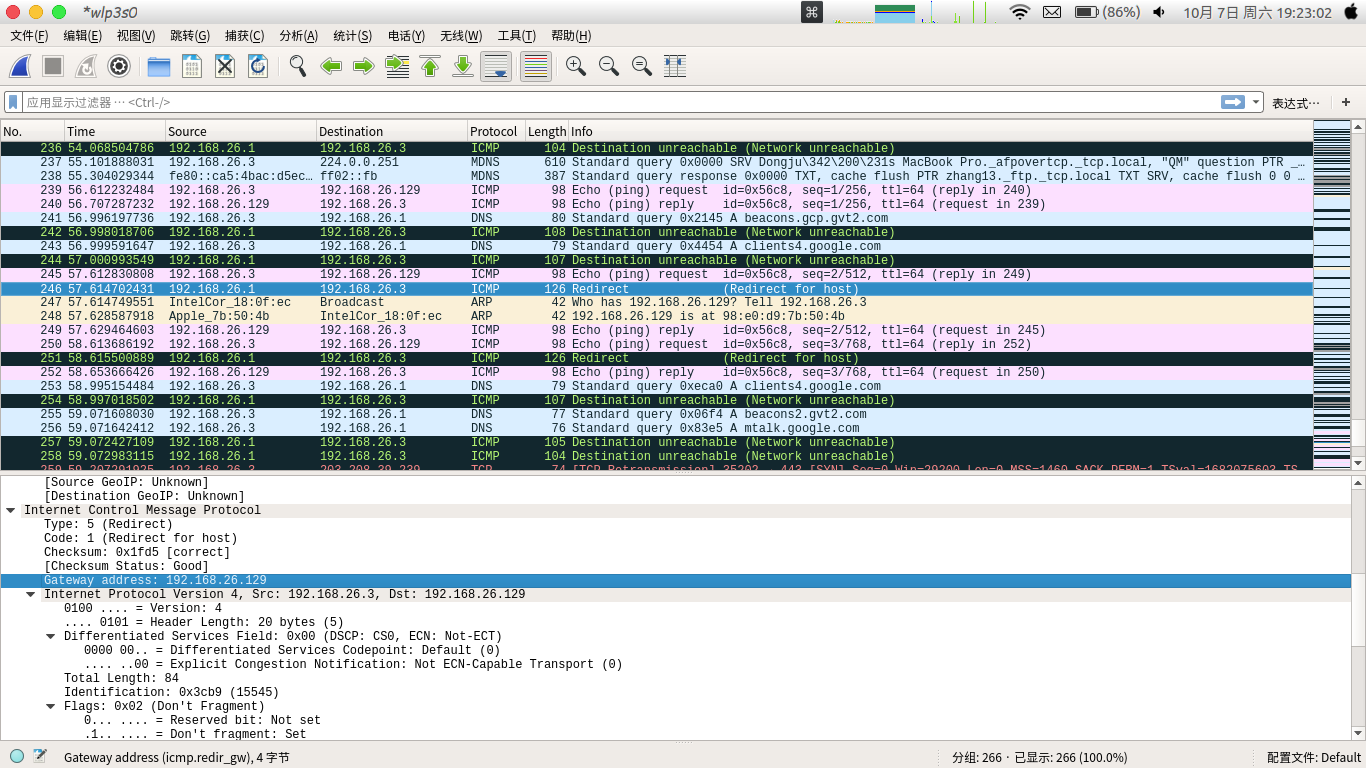
\includegraphics[width=1.0\linewidth]{redirect.png}
\caption{Redirect}
\label{fig:2}
\end{figure}

\begin{figure}[htp]
\centering
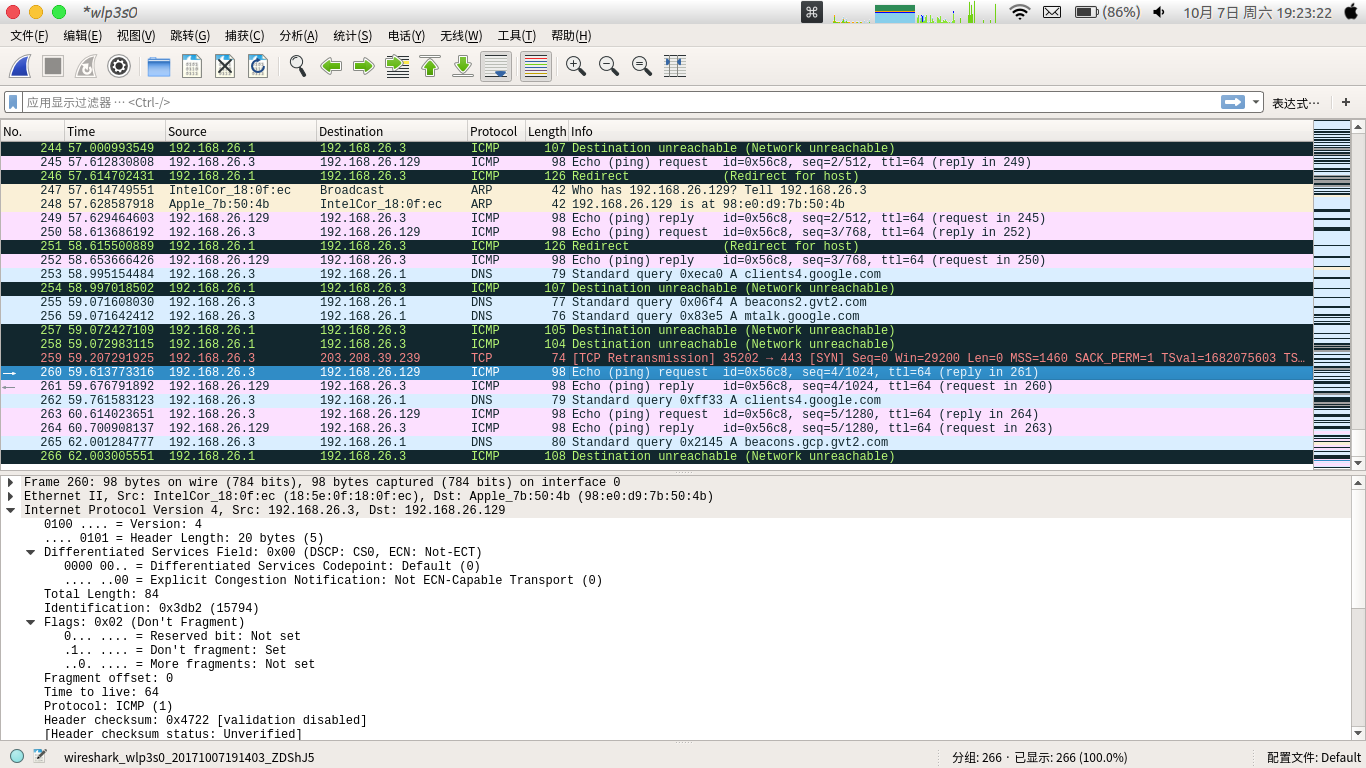
\includegraphics[width=1.0\linewidth]{ping-after.png}
\caption{重定向之后的数据}
\label{fig:3}
\end{figure}

\subsection{实验现象解释}
正常情况下(比如老师课上解释了一下),A能ping通B,B不能ping通A,我用自己的openwrt路由器试了下确实是这个样子。A能够ping通B的原因是,A使用子网掩码\uline{255.255.255.0},发现B和自己是同一个子网内的,于是直接把包发给B;B不能够ping通的原因是,B使用子网掩码\uline{255.255.255.224},发现A和自己不在同一个子网内,于是将数据包发给了网关,而不是发给A。正常情况下网关就把包丢了。

在该试验中,实验现象与结论明显不符,网关回复ICMP Redirect信息。原因是路由器有些智能,发送了重定向的数据包(见图\ref{fig:2}),告诉192.168.26.3,网关就是192.168.26.129,以后直接把数据发给这个地址。将图\ref{fig:1}和图\ref{fig:3}进行对比,可以发现数据包的第二行Ethernet发生了改变,具体为Dst的Mac地址发生改变。
\section{问题2}
在清华校园网无线网络环境下(SSID 为 Tsinghua) A用校园网账号登录了,B在A的附近连接了同一个WiFi路由器,但没有登录TUNET。 B用什么办法获得A的MAC 和IP? 如果B修改自己的IP和MAC假冒A的身份,可以做什么?
\subsection{实验步骤}
\begin{enumerate}
	\item ifconfig获取本机当前ip,为\uline{183.172.152.237/21}
	\item traceroute www.baidu.com获取网关,为\uline{183.172.152.1}
	\item nmap -sP -PI -PT -oN ipandmaclist.txt 183.172.152.1/21 扫描同一网段下的设备IP和Mac地址,结果见文件\uline{ipandmaclist.txt}(我了解到哪怕设备离得很近,连接同一个AP,也有可能不在同一信道内,Tsinghua有5个信道,因此距离近并不能够直接入侵?)
	\item ifconfig wlp3s0 down
	\item ifconfig wlp3s0 hw ether 某个Mac地址
	\item ifconfig wlp3s0 up
	\item 重新连上Tsinghua,查看\url{http://net.tsinghua.edu.cn/}页面,结果见图\ref{fig:4}
\end{enumerate}

\begin{figure}[htp]
\centering
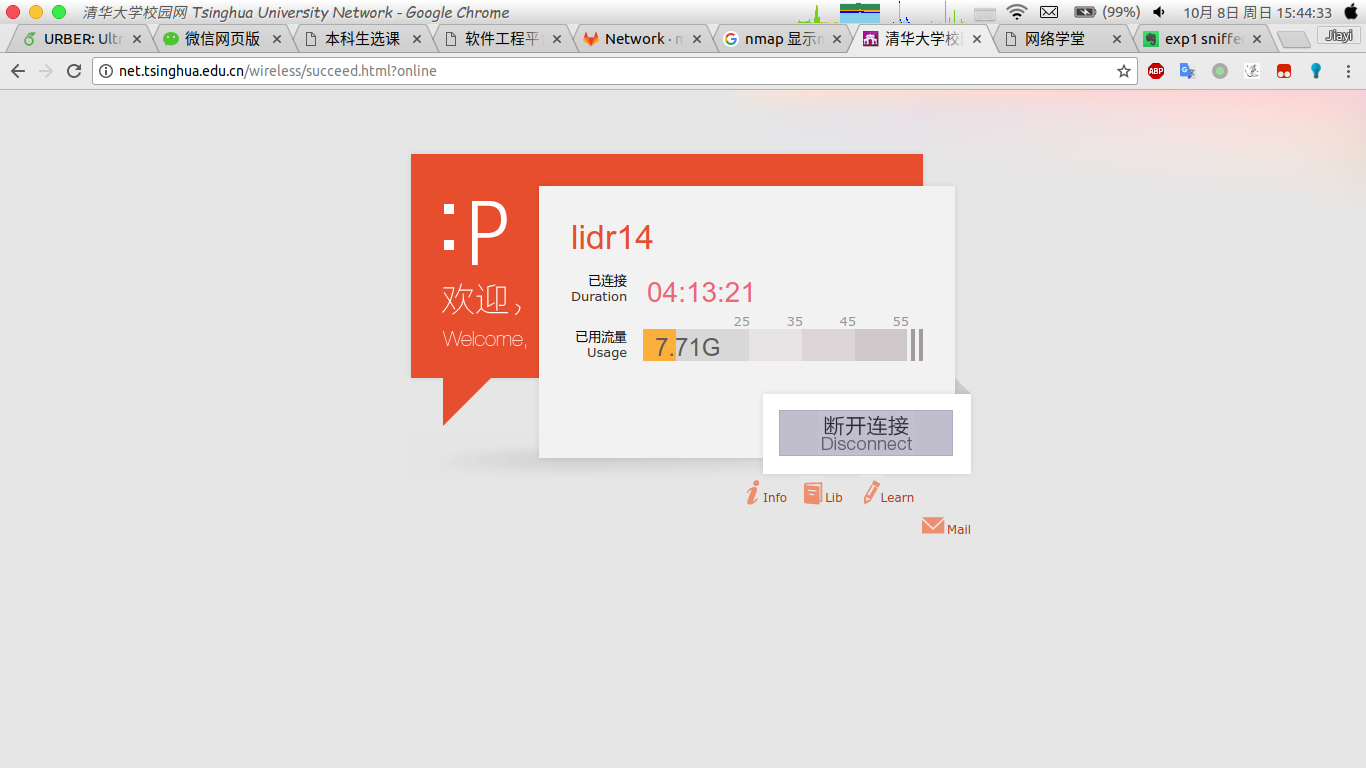
\includegraphics[width=1.0\linewidth]{lidr14.png}
\caption{某个学长(姐?)的联网信息}
\label{fig:4}
\end{figure}

如果将自己电脑的Mac改成别人的Mac,会造成联网冲突,也就是我和对方只有一个人能够上网,并且是开始联网时间靠后的设备具有优先权。如果能够做到流量转发的话,就能够暗中观察,偷走流量。如果设备连接校园网的话,似乎没有什么很好的措施能够避免这种攻击,只能手动把对方ip踢下线。

\end{document}
